\documentclass[11pt,british]{report}
\renewcommand{\rmdefault}{ptm}
\renewcommand{\familydefault}{\rmdefault}
%formatting packages
\usepackage[T1]{fontenc}
\usepackage[latin9]{inputenc}
\usepackage[a4paper]{geometry}
\geometry{verbose,tmargin=3cm,bmargin=3cm,lmargin=3.5cm,rmargin=2.4cm}
\usepackage{fancyhdr}
\pagestyle{fancy}
\setcounter{secnumdepth}{3}
\usepackage[british]{babel}
\usepackage{booktabs}
\usepackage{array,multirow}
\usepackage{subfig}
\usepackage[explicit]{titlesec}
\usepackage{adjustbox}
\usepackage{cite}
\usepackage{pdfpages}
\usepackage{standalone}
\usepackage[toc,page]{appendix}
\usepackage{listings}
\usepackage{setspace}
\usepackage{acro}
\usepackage{etoolbox}

%%maths
\usepackage{units}
\usepackage{siunitx}
\usepackage{amsmath}
\usepackage{amssymb}
\usepackage{mathrsfs}
%\usepackage{commath}
\usepackage{cancel}
\usepackage{gensymb}
\usepackage{esint}
\usepackage{mdsymbol}
%\usepackage{eurosym} 
%\usepackage{wasysym}

%%figures
\usepackage{graphicx}
\usepackage{esvect}
\usepackage{color}
\usepackage{xcolor}
\usepackage{float}
\usepackage{caption}

%\usepackage{tikz}

\usepackage[
	unicode=true,pdfusetitle,
	bookmarks=true,bookmarksnumbered=false,bookmarksopen=false,
	breaklinks=true,pdfborder={0 0 0},backref=page,colorlinks=false
	]{hyperref}

\makeatletter

\newenvironment{dedication}
{\clearpage           % we want a new page
	\thispagestyle{empty}% no header and footer
	\vspace*{\stretch{1}}% some space at the top 
	\itshape             % the text is in italics
	\raggedleft          % flush to the right margin
}
{\par % end the paragraph
	\vspace{\stretch{3}} % space at bottom is three times that at the top
	\clearpage           % finish off the page
}

%%%% ACRONYMS %%%%
\DeclareAcronym{FPGA}{
	short = FPGA, 
	short-indefinite = an,
	long = Field Programmable Gate Array
}
\DeclareAcronym{ADPLL}{
	short = ADPLL, 
	short-indefinite = an,
	long = All-Digital Phase Lock Loop
}
\DeclareAcronym{PLL}{
	short = PLL, 
	long = Phase Lock Loop
}
\DeclareAcronym{VCO}{
	short = VCO, 
	long = Voltage Controlled Oscillator
}
\DeclareAcronym{LF}{
	short = LF, 
	long = Loop Filter
}
\DeclareAcronym{PFD}{
	short = PFD, 
	long = Phase Frequency Detector
}
\DeclareAcronym{PD}{
	short = PD, 
	long = Phase Detector
}
\DeclareAcronym{UCD}{
	short = UCD, 
	long = University College Dublin
}
\DeclareAcronym{ASIC}{
	short = ASIC, 
	short-indefinite = an,
	long = Application Specific Integrated Circuit
}
\DeclareAcronym{SOC}{
	short = SoC, 
	short-indefinite = an,
	long = System-On-Chip
}
\DeclareAcronym{IOT}{
	short = IOT, 
	long = Internet Of Things
}
\DeclareAcronym{GSLS}{
	short = GSLS, 
	long = Globally Synchronous Locally Synchronous
}
\DeclareAcronym{GALS}{
	short = GALS, 
	long = Globally Asynchronous Locally Synchronous
}
\DeclareAcronym{IC}{
	short = IC,  
	long = Integrated Circuit,
	long-plural = s
}
\DeclareAcronym{CPU}{
	short = CPU, 
	long = Central Processing Unit
}
\DeclareAcronym{CMOS}{
	short = CMOS, 
	long = Complementary Metal Oxide Semiconductor
}
\DeclareAcronym{DCO}{
	short = DCO, 
	long = Digitally Controlled Oscillator
}
\DeclareAcronym{NCO}{
	short = NCO, 
	long = Numerically Controlled Oscillator
}
\DeclareAcronym{TDC}{
	short = TDC, 
	long = Time to Digital Converter
}
\DeclareAcronym{TDL}{
	short = TDL, 
	long = Tapped Delay Line
}
\DeclareAcronym{PI}{
	short = PI, 
	long = Proportional Integral
}
\DeclareAcronym{IIR}{
	short = IIR, 
	long = Infinite Impulse Response
}
\DeclareAcronym{FIR}{
	short = FIR, 
	long = Finite Impulse Response
}
\DeclareAcronym{HDL}{
	short = HDL, 
	long = Hardware Description Language
}
\DeclareAcronym{RAM}{
	short = RAM, 
	long = Random Access Memory
}
\DeclareAcronym{EDA}{
	short = EDA, 
	long = Electronic Design Automation
}
\DeclareAcronym{RF}{
	short = RF, 
	long = Radio Frequency
}
\DeclareAcronym{C2C}{
	short = C2C, 
	long = Cycle-to-Cycle
}
\DeclareAcronym{TIE}{
	short = TIE, 
	long = Time Interval Error
}
\DeclareAcronym{RADAR}{ %TODO no list
	short = RADAR, 
	long = RAdio Detection And Ranging
}
\DeclareAcronym{MSB}{
short = MSB, 
long = Most Significant Bit
}
\DeclareAcronym{Nexys}{ %TODO no list
short = Nexys4, 
long = XC7A100T-1CSG324C
}
\DeclareAcronym{RO}{ 
short = RO, 
long = Ring Oscillator
}
\DeclareAcronym{RTL}{ 
short = RTL, 
long = Register Transfer Level
}
%%%% ACRONYMS %%%%

\fancyhead{}
\fancyhead[LE,RO]{\slshape \nouppercase{\rightmark}}
\fancyhead[LO,RE]{\slshape \nouppercase{\leftmark}}
\fancyfoot[C]{\thepage}

\newcommand\T{\rule{0pt}{2.6ex}}       % Top strut
\newcommand\B{\rule[-1.2ex]{0pt}{0pt}} % Bottom strut

\preto\chapter\acresetall

\@ifundefined{showcaptionsetup}{}{%
 \PassOptionsToPackage{caption=false}{subfig}}

%\graphicspath{{Front_matter//Front_matter_images//},{Chapter_2/Chapter_2_Images//},{Chapter_3/Chapter_3_Images//},{Chapter_4/Chapter_4_Images//},{Chapter_5/Chapter_5_Images//}}

\makeatletter
\newcommand{\customlabel}[2]{%
   \protected@write \@auxout {}{\string \newlabel {#1}{{#2}{\thepage}{#2}{#1}{}} }%
   \hypertarget{#1}{#2}
}
\makeatother

%\newenvironment{dedication}
%  {\clearpage           % we want a new page
%   \thispagestyle{empty}% no header and footer
%   \vspace*{\stretch{1}}% some space at the top 
%   \itshape             % the text is in italics
%   \raggedleft          % flush to the right margin
%  }
%  {\par % end the paragraph
%   \vspace{\stretch{3}} % space at bottom is three times that at the top
%   \clearpage           % finish off the page
%  }

\begin{document}

\begin{titlepage}
	\pagenumbering{gobble}
	\setstretch{1.25}
	\begin{spacing}{3}
		\noindent \begin{center}
		{\huge{}Implementation of ADPLL Networks on FPGAs}
		\par\end{center}{\huge \par}
	\end{spacing}
	\bigskip{}
	\begin{center}
		{\Large{}Conor Dooley}
	\end{center}
	\vspace{1.25cm}
	\begin{center}
		\includegraphics[width=0.2\paperwidth]{UCD_crest.pdf}\vspace{0.25cm}
	\end{center}
	\bigskip{}
	\begin{center}
		{\large{}This thesis is submitted to the School of Electrical and Electronic Engineering\\ \vspace{0.5cm}
		in the College of Engineering and Architecture of University College Dublin \\ \vspace{0.5cm}
		in partial fulfilment for the requirements for the degree of \\ \vspace{0.5cm}
		\textbf{Master of Engineering} }
	\end{center}
	\vspace{1.cm}
	{\Large{}\bigskip{}
	\bigskip{}
	}{\Large \par}
	\noindent
	\begin{center}
		\begin{tabular}{lll}
			\textbf{\large{}Research Supervisors:} & \qquad{}\qquad{} & {\large{}Dr Elena Blokhina \& Brian Mulkeen}\\
			&  & \\
			\textbf{\large{}Head of School:} & \qquad{}\qquad{} & {\large{}Prof Andrew Keane}\\
		\end{tabular}
	\par\end{center}
	
	\vspace{1cm}
	\noindent
	\begin{center}
		{\large{}April 2019}
		\par
	\end{center}{\large \par}
\end{titlepage}

%\pagenumbering{gobble}
%\pagebreak{}

%\setstretch{1.8}
%\newpage \vspace*{7.5cm}
% Sets a PDF bookmark for the dedication
%\pdfbookmark{Dedication}{dedication}
%\thispagestyle{empty}
%\begin{center}
 % \Large \emph{}
%\Large \emph{}
%\end{center}
%\pagebreak{}

\setcounter{page}{1} 
\pagenumbering{roman}
\setstretch{1.05}
\phantomsection
\addcontentsline{toc}{chapter}{\contentsname}
\fancyhead{}
\fancyhead[LO]{\slshape \nouppercase{Contents}}

\tableofcontents{}
\listoffigures %TODO https://tex.stackexchange.com/questions/67745/remove-citation-from-list-of-figures
\listoftables

\pagebreak{}

%\begin{dedication}
%Dedicated to google and wikipedia  
%\end{dedication}

%\setcounter{page}{1} 
%\pagenumbering{roman}

%\addtocontents{toc}{\protect{\pdfbookmark[0]{Abstract}{toc}}}
%\pagestyle{empty}
%\addcontentsline{toc}{chapter}{Abstract}
%\phantomsection

\pagestyle{plain}

\setstretch{1.3}
%\chapter*{Acknowledgements } \addcontentsline{toc}{chapter}{Acknowledgements }
%\input{ackns.tex}

\chapter*{Acronyms} \addcontentsline{toc}{chapter}{Acronyms}
\printacronyms

\doublespacing
\chapter*{Abstract} \addcontentsline{toc}{chapter}{Abstract}
\documentclass[11pt,english,british]{report}
\usepackage[a4paper]{geometry}
\geometry{verbose,tmargin=3cm,bmargin=3cm,lmargin=3.5cm,rmargin=2.4cm}
\begin{document}
Low power, high frequency clock distribution systems will be in ever increasing demand in the near future as the need for high performance digital circuitry grows. At these frequencies, however, the conventional clock distribution systems are unable provide a clock signal of adequate quality without compromising on either of these problems. Many devices have turned away from using Globally Synchronous clock distribution systems in favour of those that divide the area of the chip into Globally Asynchronous but Locally Synchronous areas. However, new technologies seek to enable the use of Globally Synchronous methods at high frequencies, one of which being the use of oscillators coupled in phase, each responsible for delivering the clock to a subregion of the chip.\\
Each oscillator forms part of a Phase Lock Loop (PLL), and in order to enable the synchronisation of the network each PLL is linked those controlling the adjacent clock regions. For a digital system it is expedient to implement these PLLs digitally as an All-Digital Phase Lock Loop (ADPLL) as this provides a number of advantages. It has been shown in theory and experimentally that this method can produce the high quality clock desired with low power consumption.\\
As the production of test chips is expensive and time consuming through simulation and validation of a design is vital, traditionally carried out for mixed signal circuitry using complex behavioural and theoretical models. For a ADPLL Network the consistency of a signal both with respect to itself, and to the other clock signals on the chip is a key performance attribute and much of the variation is due to random processes that may be difficult to simulate effectively.\\
This thesis will demonstrate that the Field Programmable Gate Array (FPGA) can be used in order to simulate, model or validate ADPLL network architectures in a cost and time effective manner, as a complement to conventional methods. The key benefit is that many system dynamics that will be seen when a network is implemented on an Application Specific Integrated Circuit (ASIC), but be overlooked in software simulations can be examined in the hardware simulation that an FPGA provides.\\
This thesis implements networks using three designs of ADPLL, each using a different architecture, and highlights the use cases to which each is best suited. The performance of each design is then analysed and this compared to the suggested use cases. Additionally the impact of more minor architectural modifications is tested and documented.
\end{document}

\chapter*{Lay Abstract} \addcontentsline{toc}{chapter}{Lay Abstract}
\documentclass[11pt,english,british]{report}
\usepackage[a4paper]{geometry}
\geometry{verbose,tmargin=3cm,bmargin=3cm,lmargin=3.5cm,rmargin=2.4cm}
\begin{document}
With the increasing proliferation of ``smart'' devices the need for low power yet high speed devices has never been greater. Each smart device contains a processor to control the device, each containing complex circuitry, requiring extremely exact synchronisation. The task of this synchronisation falls to the ``clock'' signal which must occur at the same instant in all areas of the processor. Conventional solutions to this problem cannot satisfy both power and speed requirements simultaneously, so designers have proposed the ADPLL Network which approaches the problem from the other side. Rather than generate the clock once and send it around the chip, which consumes a large amount of power, an ADPLL network divides the chip into a grid and generates many signals that each serve a local area, only requiring non time critical control signals to be sent over large distances.\\
The production of chips to test designs is both expensive and time consuming so designers must ensure that mistakes have not been made, accomplished by simulating the behaviour of the designs using complex behavioural and theoretical models. This thesis will discuss the use of Field Programmable Gate Arrays (FPGA) as a hardware testing, simulation and validation platform, to be used prior to test chip production, that is both cost and time effective. The hardware nature of an FPGA enables the analysis of behaviours that would not be possible in software, without the cost and time penalties of a custom chip. This is made possible by the ability to reconfigure the chip at will, albeit with comparatively lesser capabilities.\\
This thesis implements networks using three designs of ADPLL, each using a different architecture, and highlights the use cases to which each is best suited. The performance of each design is then analysed and this compared to the suggested use cases. Additionally the impact of more minor architectural modifications is tested and documented.
%what do I do?
\end{document}

\clearpage

\pagenumbering{arabic}

\setcounter{page}{1} 
	
\pagestyle{fancy}

\fancyhead{} 

\fancyhead[LE,RO]{\slshape \nouppercase{\rightmark}} 

\fancyhead[LO,RE]{\slshape \nouppercase{\leftmark}}

\setcounter{chapter}{0}

\chapter{Introduction}\label{chap:1}
This thesis will propose the \ac{FPGA} as a tool in the design of \ac{ADPLL} networks, to bridge the gap between software simulations and implementation in custom silicon, by providing a hardware-based simulation, modelling and validation platform. While an FPGA lacks the direct control over the schematic and layout that \iac{ASIC} provides, the hardware nature of this platform enables the analysis of system dynamics that are not easily modelled in simulation and testing. \acp{ADPLL} are an entirely digital implementation of \iac{PLL}, advantageous as this allows for easier integration into the modern high transistor count \acl{IC} (\acs{IC}s) for which \ac{ADPLL} networks are a proposed clock distribution system.

The goal of this project is to design and implement an extensible platform that can be used by the research team in \ac{UCD} going forward, as they seek to understand the behaviour of \ac{ADPLL} networks at a higher level and to serve as a hardware test-bed for proposed new architectures or system components. In order to accomplish this goal, a number of potential \ac{ADPLL} architectures will be investigated, implemented and tested to ensure they function correctly. Individual \acsp{ADPLL}, however, will not give sufficient insight into the behaviour of a network, so once the \ac{ADPLL} designs have been established, each will be implemented as part of a network of increasing sizes. Each contrasting design will be analysed based on the results of measurements and tests, and these results will be used to corroborate claims made regarding which \ac{FPGA} based \ac{ADPLL} design or \ac{ADPLL} network architecture is best suited for particular use cases.

The design of each block, or component part, used in the network will be discussed, starting with the reasons for their selection and an explanation of the design methodology, along with any major pitfalls encountered in their creation. The impact on performance caused by modifications in the design of these blocks will again be assessed on the basis of measurement results, before comparison is made to both theoretical expectations and their use case.

\Iac{FPGA} based test platform is ideal for those who wish to examine system dynamics without the time delays, financial burden or expertise required to develop a complete mixed-signal system on \iac{ASIC}, yet simultaneously retaining the ability to realistically simulate the behaviour of \iac{ADPLL} network. The result of this project is such a platform, designed to be extensible, with flexibility built into each component/module used.

\setcounter{chapter}{1}

\chapter{Background Review}\label{chap:2}

\section{Brief Overview}
In a world where the demand for high performance hand-held computing devices continues to grow and the prevalence of ``smart'' devices is increasing, there is unprecedented demand for \ac{SOC} devices to control systems as varied as medical devices, watches and entertainment systems.
As these applications become more and more demanding, with ever increasing amounts of data to process and the expectation that today's devices will outperform those of yesterday, the problem of maintaining the steady gain in performance of \acp{SOC} remains at the fore.

The main drivers of performance in \acp{SOC} are the number of transistors on a chip, which is correlated with the number of calculations that can be carried out simultaneously, and the frequency at which the device operates, which determines the number of calculations performed per second.
Moore's Law, based on the famous observation by Gordon Moore in 1965\cite{moore1965cramming}, predicted a doubling in the transistor count of \aclp{IC} (\acsp{IC}) per year for the forthcoming decade. This behaviour has carried on to this day as a result of the ever decreasing size of transistors, and has only begun to slow down in recent years \cite{ross2008cpu}.
However, as the number of transistors on a chip has increased roughly following Moore's Law, the increase in clock frequency has not been able to follow a similar linear trajectory, having remained roughly equivalent for the last number of years \cite{ross2008cpu}, indeed the clock speed of the Intel Core family of \acl{CPU} (\acs{CPU}s) has not changed since their introduction in 2009 \cite{intelark}, as shown in Figure \ref{fig:eldar_last_30_yrs}
.
\begin{figure}[h]
	\centering
	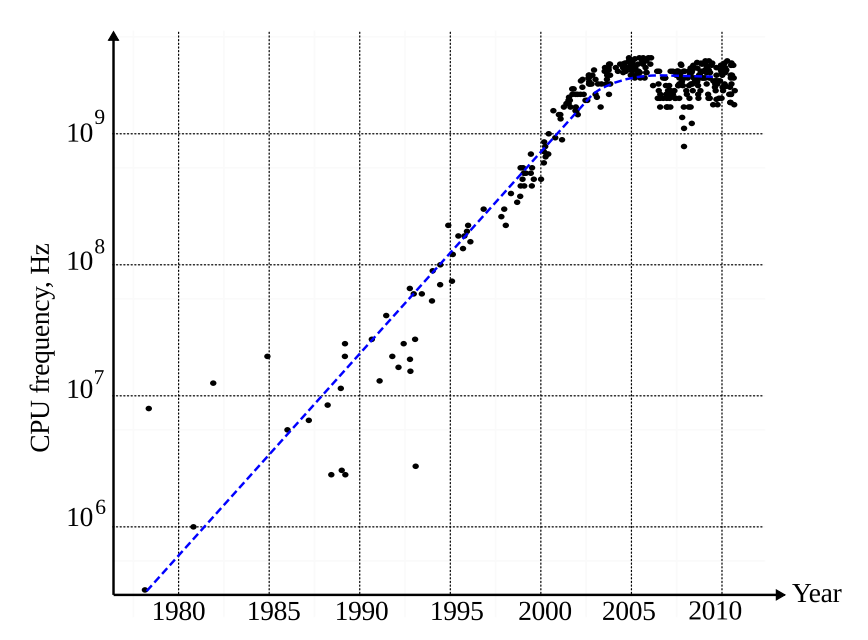
\includegraphics[scale=0.4]{../eldar_last_30_yrs}
	\caption[Frequency of the Intel microprocessors over past 30 years]{Frequency of the Intel microprocessors over past 30 years \cite{zianbetov2013phd}.}
	\label{fig:eldar_last_30_yrs}
\end{figure}\\
This plateauing of clock frequency has been caused by high power consumption, due to the demands placed by the global distribution of a high frequency clock, often the single biggest consumer of power on the chip \cite{tiwari1998reducing}.
With the growth of the \ac{IOT} market where low power devices are essential, with many of the emerging uses of \acp{SOC} being portable and thus without a permanent power source, high power consumption goes directly against one of the key pillars of the technology. This forces many of these devices to use lower performance hardware in order to reduce the power consumption, and increase their battery life,.

In digital systems, two main approaches are used when designing the clocking system. In both cases, the chip is broken down into small areas in which all transistors are clocked synchronously, with the size constrained by the ability to deliver a quality clock signal to all transistors. The first of these methods is \ac{GSLS}, where the clock signals in each of these subregions of the chip are synchronised with one other. In practice, however, this is very difficult to achieve, as extremely high precision is required across the ever increasing number of transistors and the entire area of the chip, and doing so leads to high power consumption.

In contrast, in \iac{GALS} clock delivery system the ``local'' areas are not synchronised with each other. This reduces the clocking system's complexity and thus the power consumption and chip area used, at the expense of communication speed between blocks. This disadvantage comes from the need to then somehow synchronise the messages being sent from one area to another to avoid message corruption.
\Iac{GSLS}, system, however, has the advantages of deterministic behaviour and greater rates of communication between clocking areas and, as such, remains a desirable system design. A number of methods which deliver \ac{GSLS} clocking exist at present, such as clock trees, as well as emerging technologies like the ADPLL network.

\section{The Impact of Clocking Errors}
In Figure \ref{fig:eldar_why_precise_clocking} the data path between two synchronously clocked registers is shown, with the circuit's function being carried out by the combinatorial network between the registers.
Each register has a setup time, which represents the amount of time that the input value to a register must remain constant before the clock edge, and a hold time, the time for which the input must remain constant after a clock edge.
\begin{figure}[h]
	\centering
	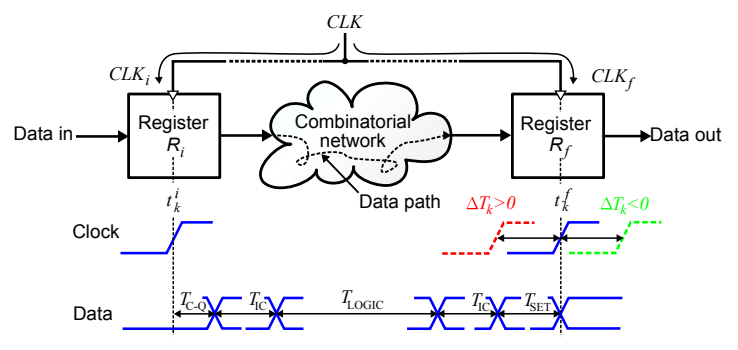
\includegraphics[scale=0.6]{../eldar_why_precise_clocking}
	\caption[Data flow in a clocked system]{Data flow in a clocked system \cite{zianbetov2013phd}.}
	\label{fig:eldar_why_precise_clocking}
\end{figure}

A lack of synchronisation between the clock edges will manifest itself as a time difference between the clocking events at both registers, $\Delta T = t^i_k - t^f_k$. $\Delta T$ is considered to be ergodic and can be described by an average deviation called skew and random process called jitter, normally modelled as a Gaussian random variable. If $\Delta T$ is negative, this reduces the time available for the intervening combinatorial network, thereby having the same effect as a reduction in clocking frequency. Correspondingly a positive $\Delta T$ for depicted registers implies a negative $\Delta T$ for $R_f$ and the subsequent register. 
The most common sources of clock error are caused by mismatches which usually stem from production, such as differences in the length of clocking paths, buffer delays or in the parameters of either active or passive components in the clock distribution network. As the size of components on \iac{IC} reduces, this mismatch becomes more difficult to avoid. All sources of mismatch will manifest themselves in the clock distribution system as skew between transistors, while the noise in active components or the power supply system will appear as jitter in the clock signal.

\section{Traditional Solutions}
A number of traditional solutions exist that produce \ac{GSLS} clocking systems, using a variety of techniques. The most simple of these implement clock distribution systems that are symmetrical in order to distribute a centrally generated clock signal to all areas of the chip at the same phase. These systems are named in accordance with their geometry, with the most common variants being branch, X or H trees. 
\begin{figure}[h]
	\centering
	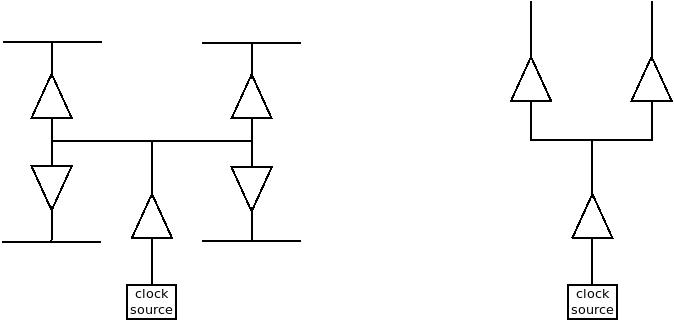
\includegraphics[scale=0.33]{../trees}
	\caption[H and branch tree clock distribution systems]{H and branch tree clock distribution systems.}
	\label{fig:trees}
\end{figure}

While on the surface these appear simple, the task of obtaining an exact matching is, in practice, the limiting factor in this design. Even if the clock distribution system is geometrically symmetrical by design, production mismatches in either active or passive components will lead to a skew that varies from part to part. In order to minimise the impact of production tolerances, the dimensions of components in the distribution network can be increased, thus reducing the relative variation possible. However this has the impact of increasing the power consumption of the distribution network \cite{tiwari1998reducing}.

A mesh clock distribution network, as in Figure \ref{fig:mesh} is an alternate design where the clock is delivered using a Cartesian grid of distribution lines. Compared to a tree type system, the variation in skew seen with a clock mesh, is inversely proportional to the density of the grid while the sources of jitter remain identical. According to Abdelhadi \textit{et al} (2010) clock meshes ``\textit{achieve low and deterministic skew, low skew variations, and low jitter}''; all desirable characteristics for a clock distribution system. However, they dissipate more power due to extra capacitive loading, attributable to the vast number of lines required to form the grid. Similarly, mesh distribution networks suffer from potential mismatch in production and alleviation, through increasing of the dimensions of interconnects, will, as with a tree type system, lead to higher power consumption \cite{abdelhadi2010timing}. 
\begin{figure}[h]
	\centering
	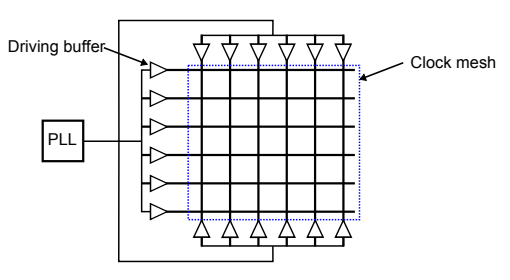
\includegraphics[scale=0.7]{../tex_files/eldar_mesh}
	\caption[Mesh clock distribution system ]{Mesh clock distribution system \cite{zianbetov2013phd}.}
	\label{fig:mesh}
\end{figure}

Alternative designs replace the electrical lines used in the tree networks with waveguides for optical signals, with only the distribution in the local area carried out using regular wires. This technique presents many advantages \cite{chen2006chip}: optical clock delivery is immune to the noise sources that affect electrical clock distribution systems, consume less power and do not suffer from the electrical losses present in a regular tree system. However, this is a fledgling method, and sufficient research into materials and potential designs has yet to be carried out \ref{zianbetov2013phd,1648640}.

\section{Skew Compensation}
In a tree type distribution system, skew is the main issue affecting clock accuracy and as such some effort has gone into addressing the problem. Skew due to the manufacturing process can be, at least, partly accounted for by means of active control through a skew compensator. This is a circuit, or controller, that compares the skew of each local clocking area on the chip and attempts to ensure in-phase clock delivery. Two main strategies exist to provide skew compensation, each named according to the location of the control mechanism. Designs featuring the controller located at the clock source, are known as ``centralised'' methods, and those with multiple controllers in the individual clocking areas are known as ``decentralised''. Regardless of the controller placement, these techniques allow for the tuning of the propagation delay between the centralised clock source and the local clocking areas.

In a centralised skew compensation circuit, the skew across the chip is calculated by the central controller, which then manipulates the distribution network in order to deliver a more in-phase clock around the chip. This calculation is done by measuring the round trip time from the clock source to both the root of the local clock tree, and to the individual ``leaves'' of the tree. The controller then has a limited ability to tune the propagation path. The downsides of this technique are that the resolution of both the measurement and compensation are poor, not permitting more than the correction of skew, and not of any jitter that may be present in the system. The extra circuitry required for both the tunability of the forward path, and the two extra return paths contributes to the increased footprint and power consumption of the distribution system.

As the name suggests a decentralised skew compensation technique, delegates the responsibility of tuning the propagation path to the individual clock regions. This strategy has the advantage of not requiring the return paths present in a ``centralised'' design. Instead, comparison is made between the leaves of different clocking areas and, on this basis, the propagation delay is varied.
For example, Yamashita \textit{et al} (2005) designed a system in which each clocking area or ``leaf node'' contains a partial clock tree. Each of these ``leaves'' is able to compare its clock phase to the neighbouring node, and based on the result, tune an adjustable delay buffer \cite{yamashita2005dynamic}. While this method can compensate for process, voltage and temperature variation, it does not address the power consumption due to the delivery of a high frequency clock across the entire chip area nor does it have any impact on clock jitter.

\section{Multi-oscillator Designs}
The designs described previously are similar, in that they have a single central oscillator that provides the clock for all areas of the chip, whereas the following methods attempt to synchronise multiple oscillators, each of which provides the clock for its own clocking area. The main advantages of a multi-oscillator design are that as each clocking area has its clock created locally, there is no degradation in the quality of the signal as it is distributed around the chip and the number of potential noise sources is reduced. In order to obtain global synchronisation some method of comparison between local clocking areas is required, and how this is done depends on the architecture. Regardless of how the comparison is made, it is carried out between neighbouring clocking areas and, therefore, the feedback network need not have a large footprint or power overhead.

One such method is a network of oscillators as in Figure \ref{fig:mizuno1998noise} which uses coupled \ac{PLL} to generate local clocks. Here the output of a leaf node is compared with an external reference and the operating frequency of each \ac{VCO} tuned based on the result.
\begin{figure}[h]
	\centering
	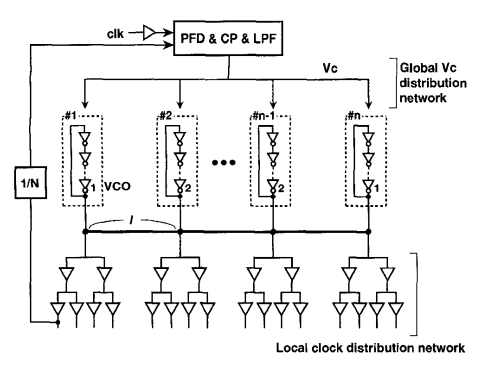
\includegraphics[scale=0.7]{../mizuno1998noise}
	\caption[Coupled oscillator clock delivery circuit]{Coupled oscillator clock delivery circuit \cite{mizuno1998noise}.}
	\label{fig:mizuno1998noise}
\end{figure}
The advantage of this method is the simplicity of the feedback network, requiring just the divided clock output from a single leaf node. The \acp{VCO} are then adjusted by the control voltage, $v_c$, which needs delivery to all areas of the chip. However, this is not a clock signal so does not suffer from skew or jitter. This alleviates the need for a power hungry distribution circuit, while also being more noise-immune than the transmission of a high frequency clock. This design does still suffer from clock variation as all \acp{VCO} are fed the same control voltage, and thus the manufacturing tolerance issues present in conventional designs persist here also. This is acknowledged by the authors:
\begin{quotation}
	\textit{Unfortunately, as with the conventional ... method, distributing the \acp{VCO} over the entire chip causes the problem that jitter and skew are increased by variations in the fabrication process (static), temperature, and power supply (dynamic)} \cite{mizuno1998noise}.
\end{quotation}
This type of multi-oscillator design is implemented by analogue circuits, and as a result not only the clock signals, but also the control signals are liable to variation due to noise, fabrication mismatch and power supply dynamics.

Another potential multi-oscillator clock distribution system uses the phase relationship between the oscillators driving neighbouring clock areas, in order to obtain synchronisation. Once again, this negates the requirement for a global distribution structure and the signals used for comparisons need only be sent between neighbouring clocking areas. As \iac{PLL} is being used, it is again possible to perform the phase comparisons using a divided version of the generated clock. This in turn means the hardware transporting the divided clock signal to the phase comparator, has significantly lower requirements placed on it, thus lowering the power consumption due to electrical losses. Pratt and Nguyen initially addressed this method of clock distribution in their 1995 paper entitled ``\textit{Distributed Synchronous Clocking}'' in which they proposed a Cartesian grid of clocking areas, each with their own \ac{PLL} This distribution method is known as \iac{PLL} Network \cite{pratt1995distributed}. In this design any given node is synchronised with its neighbours and one of the corner nodes is additionally synchronised with the reference. According to the authors, this is ``a simple, effective way to achieve low cost, high quality, low skew clock generation in a synchronous parallel processor''. They did, however, note the presence of a phenomenon called ``mode locking'', which is the settling of the network into a stable equilibrium where there are non-zero relative phases.

\begin{figure}[h]
	\centering
	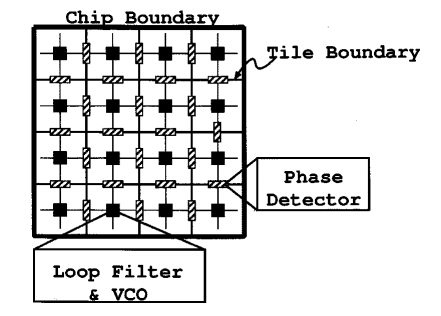
\includegraphics[scale=0.7]{../gutnik2000active}
	\caption[PLL network topology ]{PLL network topology \cite{gutnik2000active}.}
	\label{fig:gutnik2000active}
\end{figure}

This architecture of clock distribution network was then implemented by Gutnik \textit{et al} (2000) who fabricated a 4x4 array of oscillators, operating at a centre frequency of 1.2 MHz. The oscillator was implemented as a voltage controlled ``nMOS-loaded differential ring oscillator'', and in order to avoid mode locking the phase detector was implemented as a highly non-linear circuit. The design was a success and the authors concluded:
\begin{quote}
	\textit{Design and measurements on this chip confirm that generating and synchronizing multiple clocks on chip is feasible. Neither the power nor the area overhead of multiple \acsp{PLL} is substantial compared to the cost of distributing the clock by conventional means} \cite{gutnik2000active}.
\end{quote}

The remaining benefits of such a clock distribution system are: as the individual oscillators have their own control signal, mismatch between different oscillators is not a factor, as they will also receive different control signals. Secondly, and unlike the conventional methods, sources of jitter in the system, for example power supply dynamics, can be accounted for. Finally, symmetry between the different oscillators is not required, again attributable to the individual control signals in use. 

\section{ADPLL Networks}
As \iac{PLL} network is an analogue circuit, its integration in a modern \ac{IC} is a barrier to usage, and, therefore, it has not been used in any commercial designs \cite{zianbetov2013distributed}. An alternative design that is more suitable for current fabrication techniques, eschews from using analogue components and, instead, implements the network of controlled oscillators using only digital circuitry, hence the name All-Digital \ac{PLL}. A 4x4 \ac{ADPLL} network was designed and prototyped in 65 nm CMOS by Zianbetov and Shan in order to test the suitability of the technique as a clock distributor \cite{zianbetov2013phd,shan2014phd}.

In this design, the oscillators are once again laid out in a Cartesian grid, with each node phase coupled to their neighbours. As this is now a digital system, the coupling is carried out using digital phase comparators, which attempt to measure the phase difference between two oscillators. Figure \ref{fig:eldar_node} shows high level detail of the architecture of both the entire clocking system and that of an individual node in the design. The digital nature of this architecture brings with it a number of advantages over traditional analogue implementations, as it can benefit from advancements in digital circuit design suites, be reconfigurable and programmable, and has a significantly greater immunity to perturbations inherent to its digital nature, as the exact voltage of signals is of no importance \cite{zianbetov2013phd}. 

This last advantage is particularly useful in a digital environment, as otherwise there is potential for clock degradation resulting from switching of transistors. The drawback of the switch to a digital architecture, however, is the presence of quantisation. Analogue designs both deliver continuous control signals to the oscillators and have a continuous phase detection capability, unlike a digital system where these actions are carried out with fixed resolution.
\begin{figure}[!h]
	\centering
	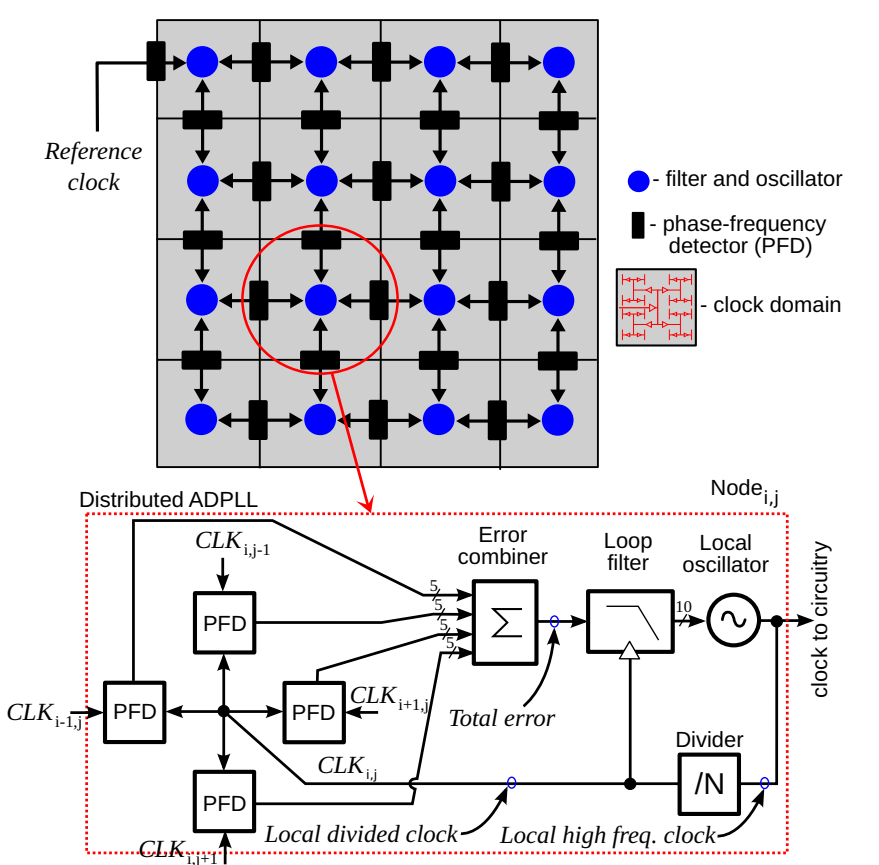
\includegraphics[scale=0.4]{../ccirc_2013_arch}
	\caption[Architecture of the ADPLL network and of a single node]{Architecture of the ADPLL network and of a single node \cite{zianbetov2013distributed}.}
	\label{fig:eldar_node}
\end{figure}
Looking at the design of a given node, it is notable that the function carried out by the Error Combiner is akin to an average, therefore as mentioned by Pratt and Nyugen, there is potential for a mode locked equilibrium in which the oscillators are not synchronised. In their paper, they presented a method where initial start-up was performed uni-directionally and, once all nodes are close to alignment, full connectivity could be restored, however this was not viable in an analogue system as reconfigurability was not an option \cite{pratt1995distributed}. Javidan \textit{et al} (2011) found that this was in fact the case, and stated:
\begin{quote}
	[Mode-locking] is solved in a simple and original way, by a dynamic reconfiguration of the network interconnection topology at the starting stage.
\end{quote}
In creating an entirely digital system, Zianbetov and Shan could easily reconfigure the network topology and, by implementing a uni-directional start-up, avoid the problem of convergence into a mode locked state, without having to design a non-linear phase detector.

\section{\acs{ADPLL} Architecture}
As indicated in Figure \ref{fig:mulkeen_pll}, the three main building blocks of a conventional \ac{PLL} are the \ac{PD}, \ac{LF} and \ac{VCO}. In \iac{ADPLL} these blocks are then replaced by their digital counterparts, necessitating quantisation in order to remain physically realisable. The ``All-Digital'' moniker is a misnomer as the oscillator and \acl{PD} are usually both implemented by mixed signal circuits.
\begin{figure}[h]
	\centering
	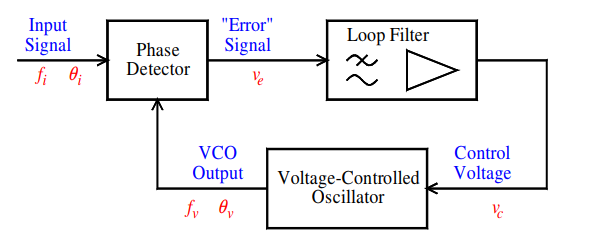
\includegraphics[scale=0.5]{../tex_files/mulkeen_pll}
	\caption[Block diagram of \iacl{PLL}]{Block diagram of \iacl{PLL}, \textit{Wireless Systems Notes}, B. Mulkeen (2017).}
	\label{fig:mulkeen_pll}
\end{figure}

\subsection{Digitally Controlled Oscillator}
In a digital system there are a very limited number of voltages representable, most commonly just two, so using a voltage to control the oscillator is not a viable strategy. Instead a fixed bit width signal is used to control the oscillator's period, selecting the number of inverters in a ring oscillator or the varactor configuration of a travelling wave oscillator \cite{chen2011rotary}. The decisions made in the design of the \ac{DCO}, or \ac{NCO}, determine many of the other \ac{ADPLL} parameters. While tuning range and centre frequency, as well as linearity, carry over from the analogue counterpart, \iac{DCO} also has a frequency step, which in combination with the bit width of the control signal determines the range over which the oscillator can be tuned. Figure \ref{fig:my_ring} illustrates a basic ring oscillator design. A ring oscillator is an inherently unstable circuit, composed of an odd number of inverters connected in a circle, which allows a signal to propagate infinitely, with the signal at any point in the circuit appearing as a square wave. The half-period of this oscillator is the time taken for the signal to propagate once through the chain, $n$ times the propagation delay through one inverter, where $n$ is the number of inverters. The frequency of operation can then be set by modulating the length of the chain, in steps of two inverters to maintain an odd number, by means of a control signal. The main impact of output frequency quantisation is that only frequencies which are at integer multiples of the frequency step away from the centre frequency can be easily reproduced. Intermediate values only obtainable in a manner akin to Fractional-N synthesis, with the control code toggling back and forth. This acts as a source of jitter in the system.
\begin{figure}[h]
	\centering
	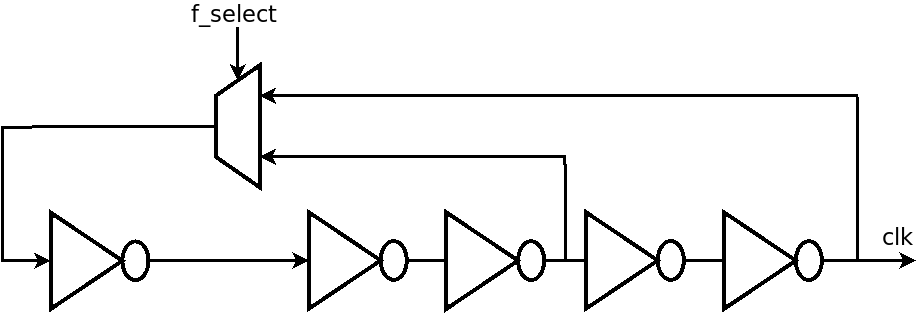
\includegraphics[width=0.6\textwidth]{../inverter_chain}
	\caption[Basic Ring/Inverter Chain Oscillator]{Basic ring/inverter chain oscillator.}
	\label{fig:my_ring}
\end{figure}

It is also possible to implement \iac{NCO} by means of a counter, in a manner that will produce either linear period or linear frequency steps. Both methods use the most significant bit of the counter's value to form the output signal. Period linearity is achieved by varying the reload value of the counter after overflow, depending on the control code, thereby changing the period by a multiple of a fixed step. Alternatively, frequency linearity can be achieved if the reload value is left constant, but instead the amount added to the counter every clock cycle is changed according to the control code, once again a fixed step size is used.

\subsection{Digital Phase Detector}
Once again quantisation impacts the \acl{PD}, as rather than a continuous output, the phase detector in \iac{ADPLL} has a finite number of output values, thus limiting the accuracy of the phase detector. A second form of quantisation is also present, as unlike an analog system, a digital phase detector does not provide continuous data in the time domain, instead relying on sampling. At its most basic, a digital phase comparator may only output an indication of which signal is leading, a design known as a Bang-Bang Detector. This can be constructed using a single D Flip Flop, with the generated signal connected to the ``D'' input and the reference signal acting as the clock. As the output only has two levels, the resultant word is only 1 bit wide, limiting the range over which the output frequency can be controlled. More complex designs, such as that in Figure \ref{fig:shan_bb_pd} implemented by Shan, build on this by measuring the time difference between edges of the signals using \iac{TDC}, in his case using \iac{TDL} \cite{shan2014phd}. \Iac{TDL} is constructed by a chain of elements of a fixed delay, and the signal to be timed is applied to this start of this chain. After the timing interval elapses the values at each point in the chain are examined, and using temperature coding, these are converted to a digital signal. The width of this signal is the bit width of the \ac{PD}'s error signal. This mimics a time measurement and allows for the phase difference to be recorded in a non binary manner.

\begin{figure}[h]
	\centering
	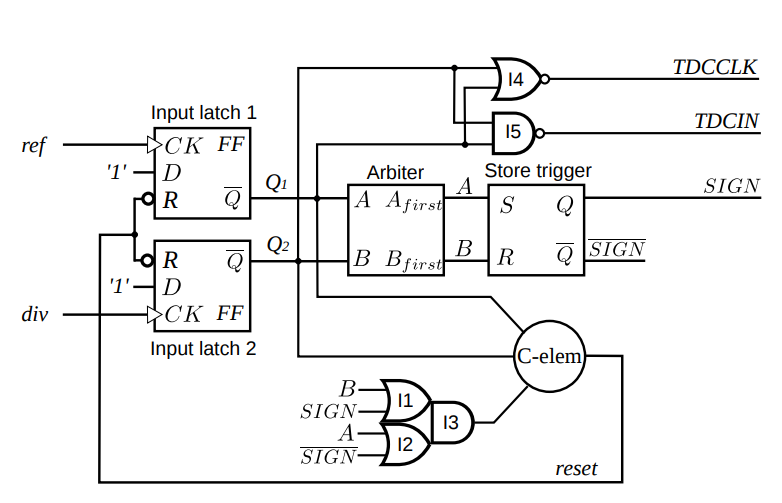
\includegraphics[width=0.65\textwidth]{../shan_bb_pd}
	\caption[Bang-bang phase/frequency detector architecture]{Bang-bang phase/frequency detector architecture \cite{shan2014phd}.}
	\label{fig:shan_bb_pd}
\end{figure}

\subsection{Digital Loop Filter}
\begin{figure}[h]
	\centering
	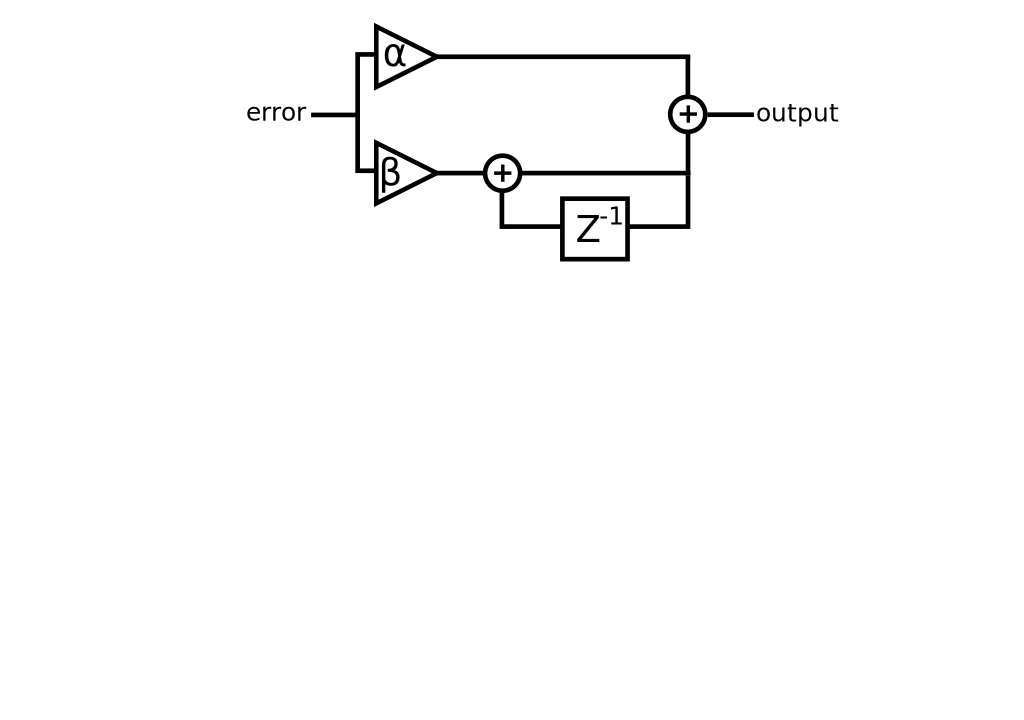
\includegraphics[width=0.6\textwidth]{../simple_pi}
	\caption[Basic \ac{PI} controller architecture]{Basic \ac{PI} controller architecture.}
	\label{fig:my_simple_pi}
\end{figure}
The \acl{LF} in \iac{ADPLL} can be implemented as \iac{PI} controller, as only a low-pass filter is required, such as that in Figure \ref{fig:my_simple_pi}. In the case of a node in \iac{ADPLL} network the input of this filter is a weighted average of the phase difference relative to the neighbouring local clocking areas. In a digital system, the proportional section can be implemented by a simple multiplier, whereas the integral path is constructed by the delayed addition of error multiplied by the integral gain to the sum of past values. This delayed accumulation can be easily implemented by an accumulator to which the current value of the multiplication is added each cycle, and as a result the system has an infinite impulse response. The value of these gains determine the response and stability of the \ac{ADPLL} network. The transfer function of such a controller is given by \cite{shan2014phd}:
\begin{equation*}
	H(z) = \alpha + \beta\frac{1}{1-z^{-1}} = \frac{(\alpha + \beta) - \alpha z^{-1}}{1-z^{-1}}\vspace{-0.2cm}
\end{equation*}
It has been found by Koskin \textit{et al} (2018), that stable operation can be achieved when the integral gain, $k_i$, is less than half the proportional gain, $k_p$ \cite{koskin2018generation}. In the same study a range of values was found which would produce low jitter operation of the network. As these values are all less than one, the filter must implement fixed point arithmetic in an effort to maintain the simplicity of the \ac{LF}, rather than incurring the penalty of floating point calculations.

\subsection{Error Combiner}
The \acp{ADPLL} used in a network need to combine the error signals from multiple neighbours to determine what the average difference from its neighbours is, and this necessitates the addition of an Error Combiner. In a digital system, this can be implemented by a weighted average of the different error signals, with the weight being modifiable at run-time. This configurability is what permits the system to implement uni-directional mode and also allows for the weighting applied to certain signals, such as the external reference, to be modified. The ease of implementation of a configurable error combiner is one of the key advantages of \iac{ADPLL} over an analogue system.

\section{The Role of the FPGA}
\Iacl{FPGA} is a type of \ac{IC} that is designed to be configured by a designer after the chip itself has been manufactured. \Iac{FPGA} contains a large number of logic elements that can be connected together in order to perform complex logic, written using the same \aclp{HDL} (\acsp{HDL}) used to design the digital blocks of \aclp{ASIC} (\acsp{ASIC}). They may also implement standard modules such as adders, multiplexers and \ac{RAM} as a fundamental element. More complex logic is often implemented using multiplexed lookup tables rather than true logic elements. High end devices such as the Xilinx Zynq Ultrascale, may implement Multi-Processor \ac{SOC}s. Compared to \iac{ASIC} the designer does not have direct control over the layout of the system but rather describes its behaviour, possibly down to the basic logic elements of inverters or other gates. Limited control is possible over the placement of the individual modules, but \ac{EDA} tools are responsible for the exact placement of elements. As a result, it is not possible to have precise control over the delays experienced as signals propagate through the design. To assist with the resolution of any issues \ac{EDA}s provide tools to analyse timing behaviour.

Prototyping on \iac{FPGA} is a common verification stage for conventional \ac{ASIC} designs, as it allows for a hardware validation of any digital circuitry, and the detection of any potential flaws or errors made by the design before the expense of \iac{ASIC} implementation. In their 2013 \ac{ADPLL} network implementation, Zianbetov and Shan used \iac{FPGA} in order to validate their programming interface, the design of the error processing block, ensure they had eliminated mode locking behaviour and to ensure phase synchronisation was possible \cite{zianbetov2013phd,shan2014phd}. However they experienced two main limitations: they were not able to implement the mixed-signal \ac{PFD} and \ac{DCO}. Secondly, the maximum frequency of operation possible was orders of magnitude lower than the GHz range of their \ac{ASIC} implementation. These issues were circumvented by implementing an alternative \ac{PFD} and \ac{DCO} designs which were driven by the clock distribution network provided by the \ac{FPGA}, and frequency scaling each clock by the same amount, such that the results of testing would remain indicative. One of the main advantages they saw was that the hardware description used for the digital blocks of their \ac{ASIC} could be directly ported over to the \ac{FPGA}.

A similar technique was used by Lata \textit{et al} (2013) to implement \iac{FPGA} clocked oscillator with a $200~\si{\kilo\hertz}$ centre frequency, however it is hard to understand exactly what either the goal was or the specifics of the \ac{DCO} used \cite{lata2013adpll}.

It is possible to implement limited mixed-signal circuits on \iac{FPGA} through the use of primitive logic elements, however, as control over the implementation is restricted to the module level, it is not possible to mirror the implementation of a design intended for \iac{ASIC}. As these implementations are analogous to a mixed-signal circuit on \iac{ASIC}, the verification of theoretical behaviours, as done by Koskin \textit{et al}, in order to test the findings of his PhD thesis \cite{theboys2019}, is made possible without the expense of \ac{ASIC} fabrication. \Iac{FPGA} based mixed-signal \ac{ADPLL} network is also seeing use here in \ac{UCD} as a initial prototyping platform for the validation of new modules for use in \ac{ASIC} based \ac{ADPLL} networks.

\ac{FPGA}s have been used in other fields to simulate and experiment with new technologies, although not all of these attempt to implement the mixed-signal circuitry using primitive elements. Fernandez-Alvarez \textit{et al} (2016) proposed a method for prototyping high-voltage system controllers suited to higher end \ac{FPGA}s in which a co-processor on the \ac{FPGA} simulates the mixed-signal circuitry while the digital section of the design is implemented on the \ac{FPGA} itself \cite{fernandez2017hw}. While the interfacing between hardware and software remains a challenge they found:
\begin{quotation}
	Obtained data are compared to the data obtained by means of using ... simulation. The proposed solution speeds up the evaluation in around one order of magnitude keeping the accuracy. The output signal differs in less than 0.6 mV (RMSD).
\end{quotation}

Mixed-signal circuits were, however, simulated in hardware by \'{O}scar Luc\'{i}a \textit{et al} (2011) on \iac{FPGA}, in order to overcome the excessive time penalty imposed by software based simulations that required the behaviour of both a digital and mixed-signal peripheral and that of a microcontroller running code in C to be simulated side by side \cite{lucia2011real}. They concluded
\begin{quotation}
	... the proposed system provides a versatile and fast method to develop ad hoc control architectures, avoiding the need for time-consuming mixed-signal simulations and the risk of damaging the actual power converter implementation.
\end{quotation}
By carrying out simulations on \iac{FPGA}, Guanhua Wang \textit{et al} (2013) achieved a 3000 times decrease in run-time when compared to an identical simulation in MATLAB used for the verification of a calibration algorithm for successive approximation analogue-to-digital converters \cite{wang2013fast}. Many other examples can be found of \ac{FPGA}s used for the simulation of mixed-signal or \acs{RF} circuits.
%TODO Elena had suggestions?

\section{\acs{ADPLL} Performance Characterisation}
As already stated, the goal of a clock distribution system is to synchronise clocking events in all areas of the chip. The effectiveness of this synchronisation is characterised by two main metrics, jitter and skew, which together describe the distribution of clocking events. Skew is the average time delay between a clocking event in one area of the chip and that of a reference event. It can be easily measured by computing the average value of this delay. Jitter has a number of definitions depending on how it is measured, but at its most basic, it is the standard deviation of the time delays with respect to the reference clocking edge.

The simplest form of clock performance characterisation is on \iac{C2C} basis, in which the reference is the previous edge of the signal under test itself. Here the standard deviation of the individual delays gives the jitter of the signal. As the previous edge of the generated signal is used as the reference, and thereby the delay is the period of the signal, the mean value is no longer the skew, but instead can be used to compute the centre frequency over the time interval. For a more informative measurement the \ac{TIE} can be computed, which takes into account another signal as the reference. \ac{TIE} is calculated by comparing the delay between the signal in question and a reference that is treated as ideal. The mean value gives the relative skew between the two signals and, once more, the standard deviation of the measurements gives the jitter with respect to this reference.

Both above forms of measurement assume a large number of sequential measurements, however, there are other ways that jitter and skew can be calculated \cite{AN10007}. Phase jitter is an important characteristic for communications systems as it can be used to calculate phase noise, important to ensure spurious emissions are within legal requirements. Long term, or accumulated, jitter represents the cumulative effect of jitter on the signal over several cycles. Long term jitter in particular affects \acs*{RADAR} as it will manifest itself as a Doppler shift in the return signal. For \iac{PLL} network, with an appropriately designed filter, the long term jitter should be zero so long as the reference signal is stable. %TODO ask Brian about this one

\setcounter{chapter}{2}

\chapter{ADPLL Designs for FPGAs}\label{chap:3}

\section{Chapter Overview}
The first step in creating an \ac{FPGA} based network of \ac{ADPLL}s is the design of the \ac{ADPLL} itself, which will be addressed in this chapter. The nature of an \ac{FPGA} necessitates a number of compromises in the design of a given block which limits transferability to \ac{ASIC} designs. In this chapter the potential designs for each individual block, or module, investigated will be explained and the case for their selection in an \ac{FPGA} based \ac{ADPLL} made. A number of blocks have implement purely digital circuitry and as such can be transferred in their entirety from an \ac{FPGA} and vice versa. However, those that will be used to emulate mixed-signal circuitry, such as the \ac{DCO} and \ac{PFD}, will be examined in greater detail.

\section{Digitally Controlled Oscillators}
The choices made in the design of the \ac{DCO} have the greatest impact on the effectiveness of the overall platform and which use cases the \ac{ADPLL} containing it are suitable for, as the key performance benchmarks are all done using the waveform this block generates. This project will address three distinct designs of \ac{ADPLL}s suitable for implementation on an FPGA, two derived from the clocks generated by the \ac{FPGA}s own distribution network and one generated independently of this clock, using a chain of inverters. These are not the only ways in which an oscillator could be synthesised on an \ac{FPGA}, however other designs were deemed to be unsuitable for extensible and portable implementations.

A prime example of this is the use of Xilinx proprietary \texttt{IODELAY} blocks to create an oscillator, as detailed in Xilinx Application Note XAPP872 \cite{iodelay}. The key idea here is that the bulk of the period is made up by the propagation time through one of the \texttt{IODELAY} blocks, which can be set at implementation time. This is combined with a section of an inverter chain, and a multiplexer used modify the length of this segment, the output of which is fed back into the \texttt{IODELAY} block. This method was discarded as the number of \texttt{IODELAY} blocks is very limited, so expanding to a larger network would be impossible, and they are all located around the edge of the chip, not suited to the construction of a Cartesian grid.

The main issue with the creation of \ac{DCO}s on an \ac{FPGA} is the inability to create mixed-signal circuits, such as those that would be intended for use on an \ac{ASIC}. As such the \ac{FPGA} based oscillator must emulate the behaviour of a mixed-signal circuit in some way.

\section{\acs{FPGA} Driven, Linear Period \acs{DCO}}
The first design of \ac{DCO} to be examined is of the type used by Zianbetov in his \ac{ADPLL} network test bed and relies on a counter driven by the clock manager on the \ac{FPGA} \cite{zianbetov2013phd}. At each event on the \ac{FPGA} provided clock a counter is incremented, overflowing upon increment past the maximum possible value. The \ac{MSB} of this counter forms the waveform generated by this oscillator, the period of which is controlled through an adjustable value that is loaded into the counter once overflow is reached, and forms the starting points for the counter. The period of oscillation is given by:
\begin{equation}
	T_{osc} = \big(2^{width} -~(BIAS+CC)~\big)\times T_{FPGA}
\end{equation}
where $T_{FPGA}$ is the clock period of the \ac{FPGA}, $CC$ is the control code input, $BIAS$ centres the oscillator in the middle of the tuning range in the event that the control code is zero and $width$ is the width of the counter used. As the only variable here is the control code, period step of this design is $T_{FPGA}$, thereby providing period linearity with respect to the control code. This is the key advantage of this design, as most \ac{ASIC} implementations of a \ac{DCO} are also linear in period. The other main reason to choose this design is that its \ac{FPGA} clocked nature allows for exact control over the frequency of operation, and the number of tunable parameters make it possible to configure multiple ways to achieve the same frequencies of operation. Combined these attributes make it very easy to create an oscillator that emulates the behaviour of a design intended for an \ac{ASIC}, however, at a greatly reduced frequency. This restriction on the frequency of operation arises out of the period step size, which in order to obtain a good resolution must be orders of magnitude smaller than the intended period to be generated. As the output waveform is taken from the counter's \ac{MSB}, the reload value of the counter must never go beyond $2^{width-1}$, as otherwise the output waveform will become a constant 1. As the reload value varies the low time of the \ac{MSB}, if the desired output waveform is a square wave this design will not be suitable.

In being \ac{FPGA} clocked this design has pseudo-deterministic characteristics, with each period step being almost identical across oscillators and over the entire tuning range, unlike an \ac{ASIC} where process variation will impact the layout of a high frequency oscillator. The only variation in this design will come, ironically, from jitter or skew in the \ac{FPGA}'s clock distribution network, which as the frequencies will typically be in the low hundreds of MHz is very minor. In the case of the Xilinx \acl{Nexys} this is at most 100 picoseconds, or 0.05\% of the period of an intended output clock at 5 MHz. To put this value into perspective, on this board the minimum value of $T_{FPGA}$ that could be used to drive this oscillator is 3.87 nanoseconds, 1.935\% of the period.

The resulting \ac{DCO} is best suited to applications that do not seek to gain a better understanding of oscillator performance, but rather those focused on validating the entirely digital blocks in the system, the role in which Zianbetov and Shan used this type of oscillator \cite{zianbetov2013phd,shan2014phd}.

\section{\acs{FPGA} Driven, Linear Frequency \acs{DCO}}
The second \ac{FPGA} clocked oscillator is similar in most attributes to the above design but eschews period linearity for frequency linearity. Again the overflow property of a counter is used with the counter's \ac{MSB} as output of the block, however, this time it forms a square wave. Rather than setting the reload value of the counter, instead the increment is adjusted depending on the control code, thus requiring $\frac{2^N}{BIAS+CC}$ increments to overflow. Accordingly the frequency of operation is set by:
\begin{equation}
	f_{osc} = f_{FPGA}\times\frac{BIAS+CC}{2^{width}}
\end{equation}
Here the control code $CC$ and bias are added to the value stored in the accumulator at each event of the \ac{FPGA}, clock until overflow is reached. This occurs at $2^{width}$ where, as before, $width$ is the bit width of the counter, thus valuing each control code increment at $\frac{f_{FPGA}}{2^{width}}$ Hz. As with the previous design, this oscillator is better suited to frequencies where the output of the \ac{DCO} is orders of magnitude lower than the clock signal driving it, as this ensures that the incremental change due to the control code remains a small fraction of the period.

This design is just as configurable as its linear-in-period counterpart, and well suited to the low frequency emulation of \ac{ASIC} based oscillators that are themselves linear in frequency. In sharing the \ac{FPGA} as a clock source again the pseudo-deterministic characteristics return, once more meaning this oscillator is better used for testing, simulating or verifying other blocks in the system.

\section{Inverter Ring \acs{DCO}}




\setcounter{chapter}{2}
%
%\chapter{Kinetic Energy Harvesters}\label{chap:3}
%
%\input{Chapter_3.tex}
%
\pagebreak{}
\phantomsection
\addcontentsline{toc}{chapter}{Bibliography}
\fancyhead[LO,RE]{\slshape \nouppercase{\leftmark}}\bibliographystyle{IEEEtran}
\bibliography{thesis}

\end{document}
